\documentclass[tikz,border=6pt]{standalone}
\usepackage[utf8]{inputenc}
\usepackage[T1]{fontenc}
\usepackage{amsmath,amssymb}
\usepackage{lmodern}
\usetikzlibrary{arrows.meta}

\definecolor{ink}{HTML}{1d1d1f}
\definecolor{sub}{HTML}{515154}
\definecolor{muted}{HTML}{6e6e73}
\definecolor{border}{HTML}{d2d2d7}
\definecolor{cardbg}{HTML}{ffffff}
\definecolor{amber}{HTML}{c76008}
\definecolor{amberbright}{HTML}{ff9f0a}
\definecolor{amberfill}{HTML}{fff3e0}
\definecolor{blue}{HTML}{0066cc}
\definecolor{bluebright}{HTML}{2997ff}
\definecolor{red}{HTML}{d70015}
\definecolor{redbright}{HTML}{ff453a}

\begin{document}
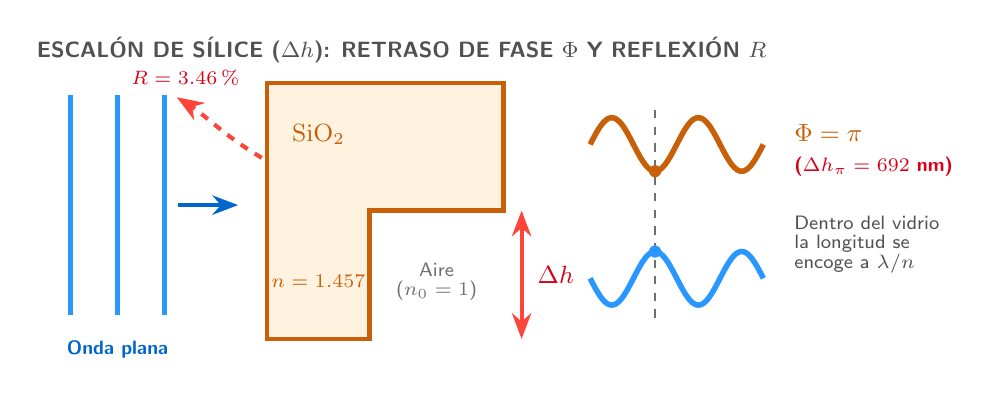
\begin{tikzpicture}[font=\sffamily,>=Stealth]

\node[anchor=west,font=\sffamily\bfseries\footnotesize,text=sub] at (0,4.52)
  {ESCALÓN DE SÍLICE ($\Delta h$): RETRASO DE FASE $\Phi$ Y REFLEXIÓN $R$};

% Onda plana incidente
\foreach \x in {0.55, 1.15, 1.75} {
  \draw[bluebright,line width=1.8pt] (\x,1.15) -- (\x,3.95);
}
\draw[->,blue,line width=1.4pt] (1.92,2.55) -- (2.68,2.55);
\node[font=\sffamily\scriptsize\bfseries,text=blue] at (1.15,0.72) {Onda plana};

% Reflexión de Fresnel en la cara anterior
\draw[->,redbright,line width=1.5pt,dashed] (2.98,3.15) .. controls (2.52,3.42) and (2.25,3.70) .. (1.90,3.92);
\node[anchor=south east,font=\sffamily\scriptsize\bfseries,text=red] at (2.82,3.94) {$R = 3.46\,\%$};

% Geometría escalón SiO2 (n=1.457) vs Aire (n0=1)
\filldraw[fill=amberfill,draw=amber,line width=1.6pt]
  (3.05,0.85) -- (3.05,4.10) -- (6.05,4.10) -- (6.05,2.48) -- (4.35,2.48) -- (4.35,0.85) -- cycle;

\node[font=\sffamily\small\bfseries,text=amber] at (3.70,3.45) {$\mathrm{SiO_2}$};
\node[font=\sffamily\scriptsize\bfseries,text=amber] at (3.70,1.58) {$n = 1.457$};
\node[font=\sffamily\scriptsize,text=muted,align=center] at (5.20,1.58) {Aire\\[-1pt]($n_0 = 1$)};

% Cota Δh
\draw[<->,redbright,line width=1.4pt] (6.28,0.85) -- (6.28,2.48);
\node[anchor=west,font=\sffamily\small\bfseries,text=red] at (6.36,1.66) {$\Delta h$};

% Ondas salientes desfasadas Phi = pi
% Onda superior (vidrio): sin(2*pi*(x-7.15)/1.1) -> ciclo 1.1 cm, máximo en 7.425
\draw[amber,line width=2.0pt,smooth,samples=90,domain=7.15:9.35]
  plot (\x, {3.32 + 0.34*sin(deg(2*pi*(\x-7.15)/1.1))});

% Onda inferior (aire): desfasada exactamente pi -> -sin(...)
\draw[bluebright,line width=2.0pt,smooth,samples=90,domain=7.15:9.35]
  plot (\x, {1.62 - 0.34*sin(deg(2*pi*(\x-7.15)/1.1))});

% Línea vertical comparando cresta vs valle
\draw[muted,dashed,line width=1.0pt] (7.975,1.12) -- (7.975,3.82);
\fill[amber] (7.975,2.98) circle (2.2pt);
\fill[bluebright] (7.975,1.96) circle (2.2pt);

% Etiquetas derecha
\node[anchor=west,font=\sffamily\small\bfseries,text=amber] at (9.62,3.46) {$\Phi = \pi$};
\node[anchor=west,font=\sffamily\scriptsize\bfseries,text=red] at (9.62,3.04) {($\Delta h_\pi = 692\text{ nm}$)};
\node[anchor=west,font=\sffamily\scriptsize,text=sub,align=left] at (9.62,2.05) {Dentro del vidrio\\[-1pt]la longitud se\\[-1pt]encoge a $\lambda/n$};

\end{tikzpicture}
\end{document}
